\documentclass[11pt]{article}
\usepackage[margin=2.5cm]{geometry}
\usepackage{amsmath,amssymb,amsthm}
\usepackage{tikz}
\usetikzlibrary{arrows.meta}
\newcommand{\cb}{\bar{\mathbf c}}
\newcommand{\bx}{\mathbf x}

\title{Numerical Verification of Theorem 3.1\\(Bertsimas \& Tsitsiklis)}
\date{}
\begin{document}
\maketitle

\noindent\textbf{Theorem 3.1.} \\ Let $\bx$ be a basic feasible solution with basis matrix $B$ and reduced costs
$\bar c_j = c_j - \mathbf c_B^\top B^{-1}A_j$.
(a) If $\cb\ge 0$, then $\bx$ is optimal.
(b) If $\bx$ is optimal and nondegenerate, then $\cb\ge 0$.

\section{The problem}
\[
\begin{aligned}
\min\quad & -x_1 - 2x_2\\
\text{s.t.}\quad & x_1 + x_2 \le 4,\quad x_1 \le 3,\quad x_2 \le 3,\quad x_1,x_2\ge 0.
\end{aligned}
\]
Adding slacks $s_1,s_2,s_3\ge 0$ gives the standard form $A\bx=\mathbf b$, $\bx\ge 0$, with variables
$(x_1,x_2,s_1,s_2,s_3)$:
\[
A=\begin{pmatrix}1&1&1&0&0\\1&0&0&1&0\\0&1&0&0&1\end{pmatrix},\qquad
\mathbf b=\begin{pmatrix}4\\3\\3\end{pmatrix},\qquad
\mathbf c=(-1,-2,0,0,0)^\top .
\]
For each basis we compute $\mathbf p^\top=\mathbf c_B^\top B^{-1}$ (i.e.\ solve $B^\top\mathbf p=\mathbf c_B$) and then
$\bar c_j = c_j-\mathbf p^\top A_j$.

\section{The polyhedron}
\begin{center}
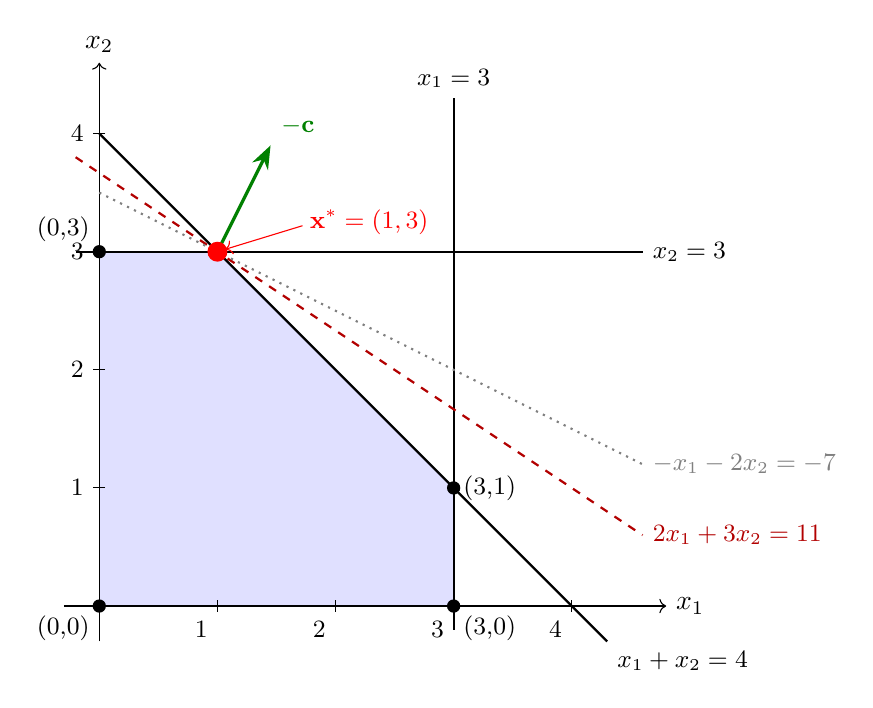
\begin{tikzpicture}[scale=1.5]
  \fill[blue!12] (0,0)--(3,0)--(3,1)--(1,3)--(0,3)--cycle;
  \draw[->] (-0.3,0)--(4.8,0) node[right]{$x_1$};
  \draw[->] (0,-0.3)--(0,4.6) node[above]{$x_2$};
  \foreach \t in {1,2,3,4}{\draw (\t,0.05)--(\t,-0.05) node[below left]{\small\t};
                           \draw (0.05,\t)--(-0.05,\t) node[left]{\small\t};}
  % constraints
  \draw[thick] (0,4)--(4.3,-0.3) node[below right]{\small $x_1+x_2=4$};
  \draw[thick] (3,-0.2)--(3,4.3) node[above]{\small $x_1=3$};
  \draw[thick] (-0.2,3)--(4.6,3) node[right]{\small $x_2=3$};
  % redundant constraint used in Section 5
  \draw[thick,dashed,red!70!black] (-0.2,{(11+0.4)/3})--(4.6,{(11-9.2)/3})
       node[right]{\small $2x_1+3x_2=11$};
  % objective level lines
  \draw[gray,dotted,thick] (0,3.5)--(4.6,1.2) node[right]{\small $-x_1-2x_2=-7$};
  \draw[-{Stealth},very thick,green!50!black] (1,3)--(1.45,3.9)
       node[above right]{\small $-\mathbf c$};
  % vertices
  \foreach \p/\l/\a in {(0,0)/{(0,0)}/below left,(3,0)/{(3,0)}/below right,
                        (3,1)/{(3,1)}/right,(0,3)/{(0,3)}/above left}
     {\fill \p circle(1.6pt) node[\a]{\small \l};}
  \fill[red] (1,3) circle(2.4pt); \node[red,anchor=west] at (1.7,3.25) {\small $\bx^*=(1,3)$}; \draw[red,->,shorten >=3pt] (1.72,3.22)--(1,3);
\end{tikzpicture}
\end{center}
Objective values at the vertices: $(0,0)\!:0$, $(3,0)\!:-3$, $(3,1)\!:-5$, $(0,3)\!:-6$, $(1,3)\!:-7$.
So $\bx^*=(1,3)$ is the unique optimum.

\section{Part (a): $\cb\ge 0$ certifies optimality}
At $\bx^*=(1,3)$: $s_1=0$, $s_2=2$, $s_3=0$. Basis $\{x_1,x_2,s_2\}$:
\[
B=\begin{pmatrix}1&1&0\\1&0&1\\0&1&0\end{pmatrix},\quad
\mathbf x_B = B^{-1}\mathbf b=\begin{pmatrix}1\\3\\2\end{pmatrix},\quad
\mathbf p=\begin{pmatrix}-1\\0\\-1\end{pmatrix}.
\]
Nonbasic reduced costs:
\[
\bar c_{s_1}=0-\mathbf p^\top e_1 = 1,\qquad \bar c_{s_3}=0-\mathbf p^\top e_3 = 1 .
\]
Hence $\cb=(0,0,1,0,1)\ge 0$, and by (a) $\bx^*$ is optimal, which agrees with the vertex table.

\paragraph{Contrast: a non-optimal BFS.} At $(3,1)$, basis $\{x_1,x_2,s_3\}$, $\mathbf x_B=(3,1,2)$ (nondegenerate),
$\mathbf p=(-2,1,0)$ and $\cb=(0,0,2,-1,0)$. Since $\bar c_{s_2}=-1<0$, increasing $s_2$ (moving along the edge
$x_1+x_2=4$ toward $(1,3)$) lowers the cost by $1$ per unit. This is consistent with (b): this BFS is nondegenerate and has
a negative reduced cost, so it cannot be optimal.

\section{Part (b): nondegeneracy matters}
The basis in Section 3 is nondegenerate ($\mathbf x_B=(1,3,2)>0$) and optimal, and indeed $\cb\ge0$, as (b) states.

To see why the hypothesis is needed, add the \emph{redundant} constraint $2x_1+3x_2\le 11$ (slack $s_4$), which is
tight only at $(1,3)$ (dashed line). The feasible set and the optimum are unchanged, but now $m=4$ and four constraints are
active at $(1,3)$, so every BFS at this point is \textbf{degenerate}. Take the basis $\{x_1,x_2,s_2,s_3\}$:
\[
\mathbf x_B=(1,3,2,\mathbf{0}),\qquad \mathbf p=(1,0,0,-1),\qquad
\cb=(0,0,\,\mathbf{-1},\,0,\,0,\,1).
\]
Here $\bar c_{s_1}=-1<0$, yet $\bx^*$ is optimal. The direction associated with $s_1$ is infeasible: with
$s_3=0$ basic, it would push $s_3$ negative, so the step length is $\theta^*=0$.

A different basis for the same point, $\{x_1,x_2,s_2,s_4\}$, gives $\cb=(0,0,1,0,1,0)\ge0$. So the optimality
certificate depends on the choice of basis: for a degenerate optimal $\bx$, some basis has $\cb\ge0$ (this is what
the simplex method finds), but not necessarily every basis.

\section{Summary}\small
\begin{center}
\begin{tabular}{lllll}
\hline
Point & Basis & Degenerate? & $\cb$ & Optimal?\\ \hline
$(1,3)$ & $x_1,x_2,s_2$ & no & $(0,0,1,0,1)\ge0$ & yes\\
$(3,1)$ & $x_1,x_2,s_3$ & no & $(0,0,2,-1,0)$ & no\\
$(1,3)$, extra row & $x_1,x_2,s_2,s_3$ & yes & $(0,0,-1,0,0,1)$ & yes\\
$(1,3)$, extra row & $x_1,x_2,s_2,s_4$ & yes & $(0,0,1,0,1,0)\ge0$ & yes\\ \hline
\end{tabular}
\end{center}
\end{document}
